\section{Resultados}
El análisis detallado del corpus literario revela las tendencias tecnológicas que definen la frontera del conocimiento en ITS y monitoreo de conductores, exponiendo una clara transición metodológica desde modelos matemáticos deterministas hacia sistemas adaptativos de redes neuronales profundas.

\subsection{Dominio de Algoritmos YOLO en Tareas de Detección}
Dentro del paradigma de Deep Learning, las arquitecturas de detección de objetos en una sola etapa (one-stage detectors) dominan la literatura de forma abrumadora debido a su capacidad de inferencia en tiempo real. Específicamente, los modelos de la familia YOLO (You Only Look Once) son la primera opción para tareas de detección en tiempo real de vehículos e infracciones. Los modelos YOLOv5 \cite{kumar2026uavbased, chen2026hybrid} continúan siendo ampliamente referenciados y adaptados debido a su madurez y facilidad de entrenamiento. Para tareas de vigilancia de tráfico a gran escala, variantes optimizadas de YOLOv5 \cite{zia2025advancing, yang2025computer} logran excelentes tasas de detección de camiones y motocicletas. Asimismo, estudios centrados en la compresión de modelos \cite{essahraui2025realtime, jing2025traffic} demuestran que la cuantización de pesos viabiliza su ejecución en hardware con recursos limitados.

Paralelamente, YOLOv8 \cite{pavan2026aipowered, essahraui2025realtime} se consolida como la arquitectura preferida para aplicaciones que demandan un alto balance entre velocidad y precisión, incorporando innovaciones como la cabeza de detección libre de anclajes (anchor-free) y una estructura de pérdida modificada. Varios investigadores han propuesto mejoras a la capa de atención de YOLOv8 \cite{satya2025utilization, le2025redlight} para mitigar la tasa de falsos negativos en condiciones de lluvia o niebla. Otros trabajos \cite{silva2025light, oussouaddi2025dsryolo} integran YOLOv8 con estimadores de velocidad basados en flujo óptico. Asimismo, versiones más recientes e híbridas como YOLOv7 \cite{liu2026research, alshehri2025integrated}, YOLOv9 \cite{xie2025yoloace}, YOLOv10  y YOLOv11  demuestran innovaciones en términos de eficiencia de parámetros y atención multiescala, permitiendo capturar vehículos a gran distancia en tomas de alta resolución espacial.

Asimismo, investigaciones muy recientes comienzan a explorar la transición desde detectores de objetos basados puramente en convoluciones hacia arquitecturas basadas en Transformers de tiempo real, tales como RT-DETR \cite{yang2025computer, essahraui2025realtime}. Estos modelos eliminan la necesidad del procesamiento posterior de Supresión No Máxima (NMS, por sus siglas en inglés), el cual suele representar un cuello de botella de latencia crítico en sistemas embebidos de tráfico cuando la densidad de vehículos es extremadamente alta \cite{lin2025dangerous, satya2025utilization}. Al procesar las relaciones espaciales mediante auto-atención multi-escala directa de manera paralela, RT-DETR y sus variantes híbridas prometen un rendimiento de detección más estable frente a oclusiones mutuas de vehículos en autopistas saturadas, abriendo una nueva línea de optimización para los sistemas inteligentes de transporte de próxima generación.

\subsection{Redes Neuronales Convolucionales y Modelos Temporales}
Las redes convolucionales clásicas (CNN) \cite{liu2026research, zambrano2026monitoring} se mantienen como la base estructurante para el análisis de fatiga y la clasificación fina de expresiones faciales a través de marcas faciales. Para robustecer la detección frente a cambios rápidos en la pose de la cabeza, se proponen redes CNN multirrama \cite{l2026safestreets, ahmad2026comparative} y modelos basados en MobileNet \cite{chen2026hybrid, zia2025advancing} optimizados para bajo consumo energético. 

Para la modelación temporal de secuencias de video (por ejemplo, el análisis continuo del comportamiento o de colisiones a lo largo del tiempo), los autores recurren a redes recurrentes y LSTM \cite{kumar2026intelligent, ahmad2026comparative}. Las arquitecturas combinadas CNN-LSTM \cite{alshehri2025integrated, ijaradar2025datadriven} permiten capturar transiciones dinámicas como el pestañeo lento o el cabeceo del conductor. Otros desarrollos \cite{duan2025multimodal, arjunan2024realtime} aplican redes de memoria para la predicción de trayectorias vehiculares en cruces urbanos. Por último, la irrupción de los Vision Transformers (ViT) y mecanismos de auto-atención \cite{kumar2026intelligent, lin2025dangerous} marca un cambio tecnológico relevante, permitiendo capturar relaciones espaciotemporales de largo alcance con mayor precisión. Modelos espaciotemporales basados en atención \cite{huang2025dtldetector, alshehri2025integrated} y transformers de escala temporal \cite{kumar2025smart, tran2024transformerbased} se posicionan como alternativas altamente precisas aunque computacionalmente costosas.

\subsection{Enfoques de Machine Learning y Arquitecturas Híbridas}
A pesar del dominio del aprendizaje profundo, los algoritmos tradicionales de Machine Learning mantienen un rol importante en el estado del arte. Los modelos SVM \cite{abarghooei2026driving, ahmad2026comparative} y Random Forest \cite{uddin2025abnormal, usman2024distracted} se emplean comúnmentmente para la clasificación final de datos tabulares provenientes de sensores a bordo del vehículo o variables fisiológicas directas. Adicionalmente, clasificadores tradicionales \cite{essahraui2025realtime, wu2024driving} y modelos basados en árboles \cite{xue2023young, dong2022fatigue} ofrecen una alta interpretabilidad requerida para sistemas de seguridad activa críticos.

Adicionalmente, las arquitecturas híbridas \cite{ahmad2026comparative, essahraui2025realtime} combinan el poder de representación de características de Deep Learning (usando CNNs como extractores automáticos de características de alto nivel) con la robustez estadística de los clasificadores ML tradicionales para reducir la latencia de inferencia y optimizar el rendimiento en hardware de borde con recursos limitados. Propuestas basadas en la extracción híbrida \cite{mota2025integration, suresh2025traffic} reducen el tiempo de entrenamiento sin sacrificar precisión. Por su parte, los enfoques tradicionales de visión por computadora  se aplican en la etapa de preprocesamiento, como la normalización del contraste y la segmentación básica de regiones de interés (ROI) mediante umbralización y descriptores geométricos básicos .

\subsection{Entornos Experimentales de Prueba y Despliegue de Hardware}
Los entornos experimentales reportados en la literatura científica para validar estas soluciones inteligentes se clasifican en cuatro áreas principales:
\begin{enumerate}
    \item \textbf{Cámaras de Videovigilancia (CCTV):} Utilizadas principalmente para el monitoreo pasivo de intersecciones urbanas, detección de infracciones y detección automática de colisiones \cite{l2026safestreets, kumar2026intelligent}.
    \item \textbf{Cámaras A bordo / Conducción Naturalista:} Conducción en vehículos reales o simuladores con cámaras de cabina \cite{liu2026research, rahman2026costeffective}.
    \item \textbf{Imágenes Aéreas (UAV / Drones):} Toma aérea de tráfico y trayectorias \cite{kumar2026uavbased, bhavsar2025evaluating}.
    \item \textbf{Simuladores de Conducción / Entornos Virtuales:} Simuladores en PC o cabinas virtuales \cite{abarghooei2026driving, zambrano2026monitoring}.
\end{enumerate}

Para profundizar en las relaciones entre el entorno experimental y las librerías o hardware utilizados, la Fig.~\ref{fig:heatmap_relacion} ilustra la concentración de trabajos mediante un mapa de calor coincidente de frecuencias. Como se observa, existe una fuerte dependencia del uso de librerías como OpenCV o MediaPipe aplicadas sobre entornos reales y CCTV \cite{ahmad2026comparative, srivastava2026traffic}, mientras que el hardware de borde especializado como las GPUs NVIDIA Jetson y Raspberry Pi representan los principales habilitadores para implementar estos sistemas directamente en vehículos reales y UAV \cite{fei2025enhancing, zuo2025composite}.

\begin{figure}[htbp]
\centerline{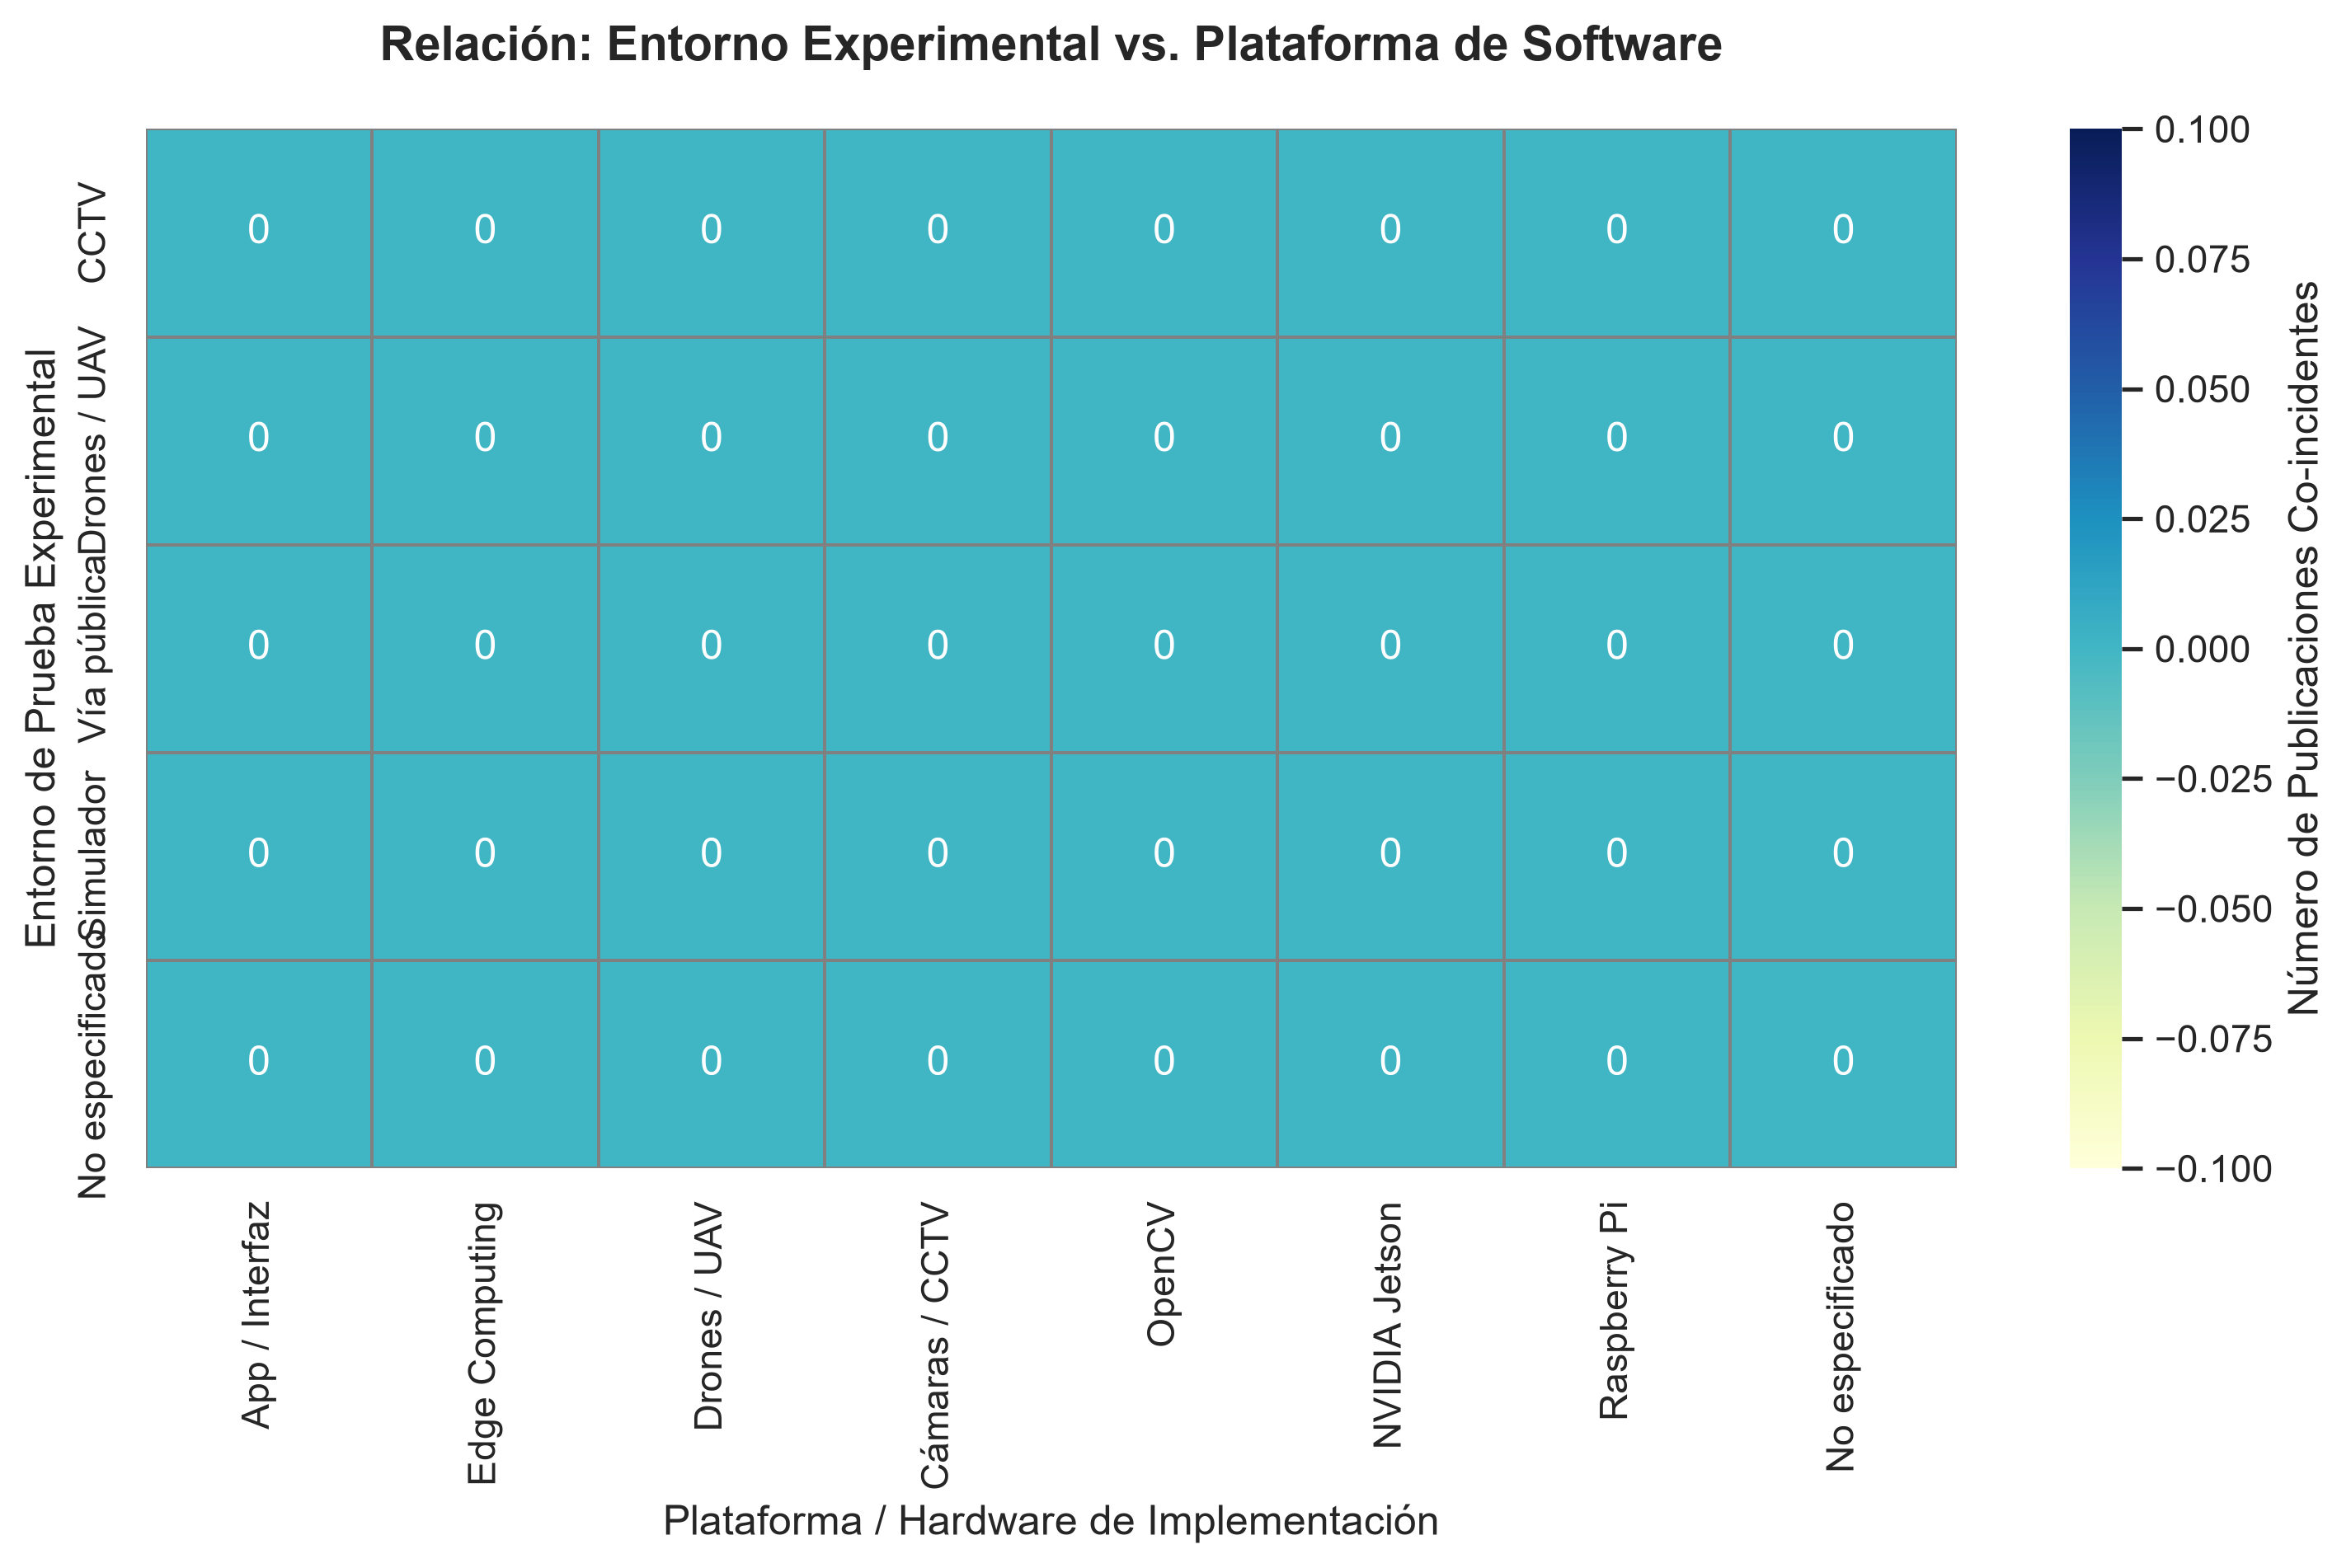
\includegraphics[width=0.48\textwidth]{../graficos/10_heatmap_relacion.png}}
\caption{Mapa de Calor Cruzado: Entorno Experimental vs. Plataforma de Implementación de Software y Hardware.}
\label{fig:heatmap_relacion}
\end{figure}

\begin{figure}[htbp]
\centerline{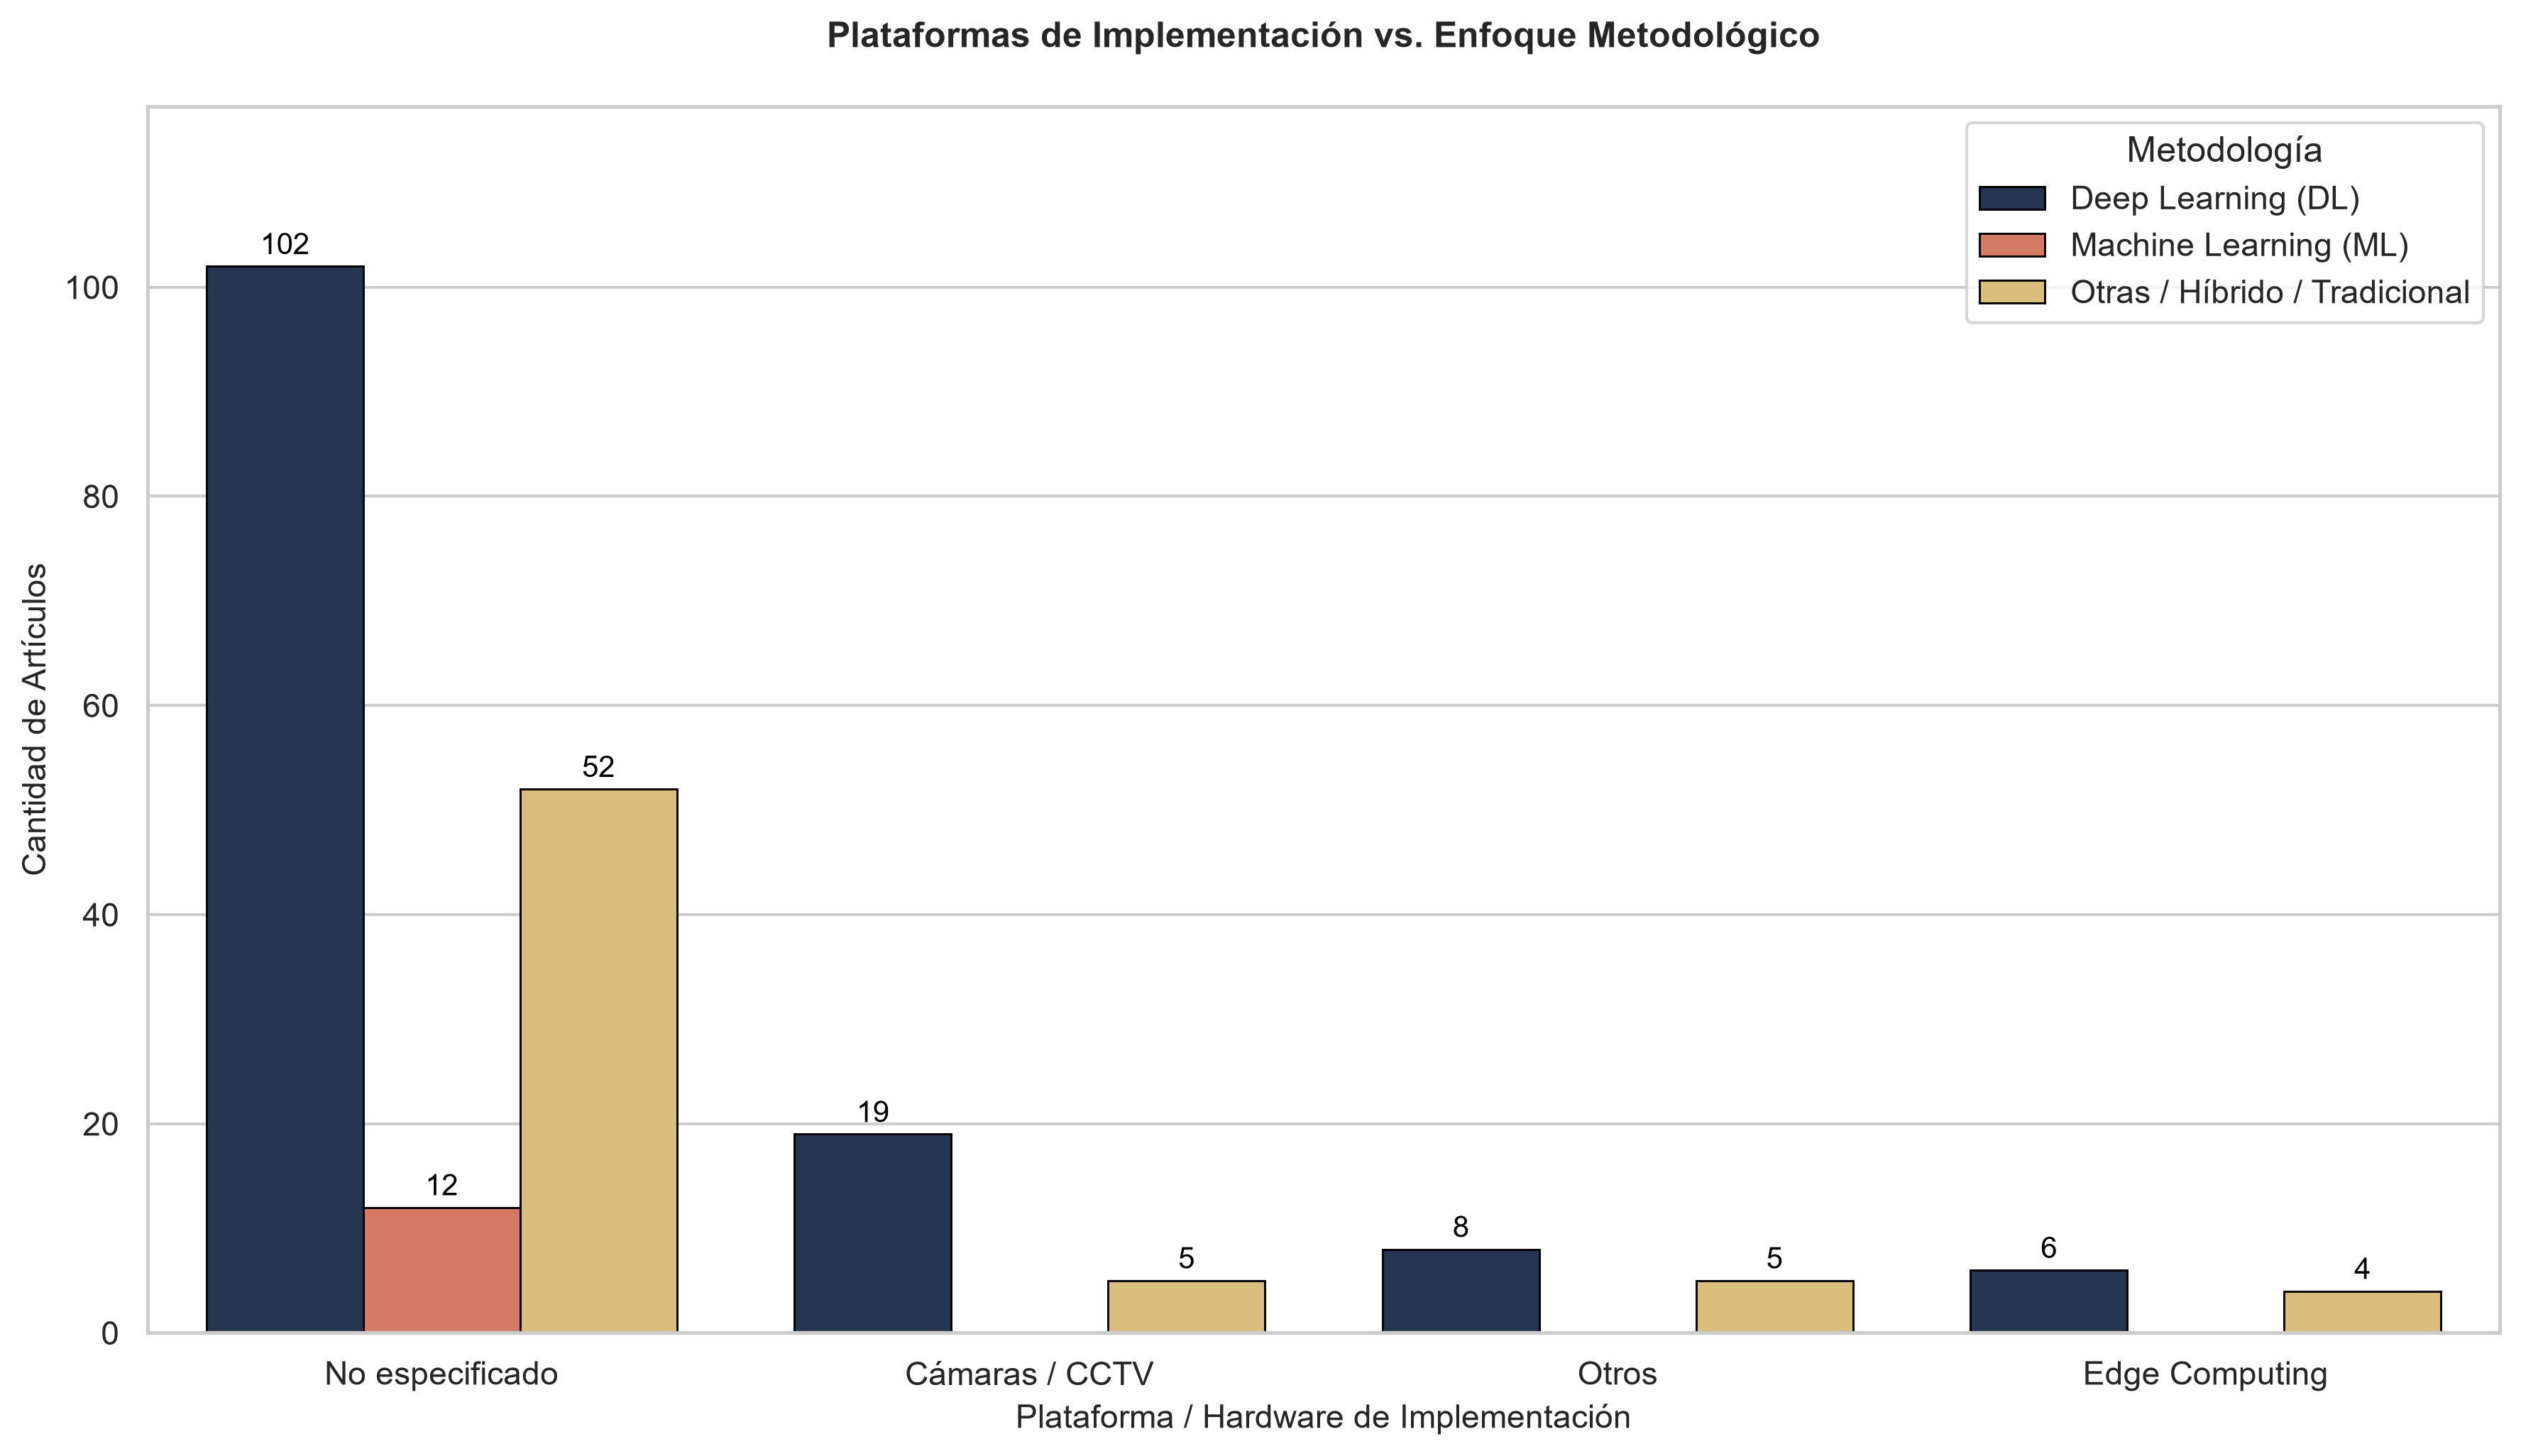
\includegraphics[width=0.48\textwidth]{../graficos/17_cruce_implementacion_metodologia.png}}
\caption{Plataformas de Implementación vs. Enfoque Metodológico de la Investigación.}
\label{fig:cruce_implementacion}
\end{figure}

\subsection{Evaluación del Rendimiento y Métricas Comparativas}
La evaluación del rendimiento de los modelos en la literatura científica se basa en métricas de clasificación y regresión bien establecidas en visión por computadora. Entre las principales se encuentran la exactitud (Accuracy), la precisión (Precision), la sensibilidad (Recall), el puntaje F1 (F1-Score) y la precisión media promedio (mAP). Las fórmulas que gobiernan estas métricas principales se definen de la siguiente manera:

\begin{equation}
\text{Accuracy} = \frac{\text{TP} + \text{TN}}{\text{TP} + \text{TN} + \text{FP} + \text{FN}}
\end{equation}

\begin{equation}
\text{Precision} = \frac{\text{TP}}{\text{TP} + \text{FP}}
\end{equation}

\begin{equation}
\text{Recall} = \frac{\text{TP}}{\text{TP} + \text{FN}}
\end{equation}

\begin{equation}
\text{F1-Score} = 2 \cdot \frac{\text{Precision} \cdot \text{Recall}}{\text{Precision} + \text{Recall}}
\end{equation}

donde TP representa los verdaderos positivos, TN los verdaderos negativos, FP los falsos positivos y FN los falsos negativos. Para evaluar cuantitativamente el desempeño de estas soluciones en base a la literatura que reporta métricas numéricas concretas, la Fig.~\ref{fig:boxplot_accuracy} expone mediante diagramas de caja y bigotes la distribución del rendimiento (\textit{accuracy}) reportado según el enfoque metodológico de IA empleado. Este análisis comparativo consolida visualmente la efectividad del aprendizaje profundo en contraste con otras aproximaciones estadísticas o híbridas \cite{fei2025enhancing, jing2025traffic}.

\begin{figure}[htbp]
\centerline{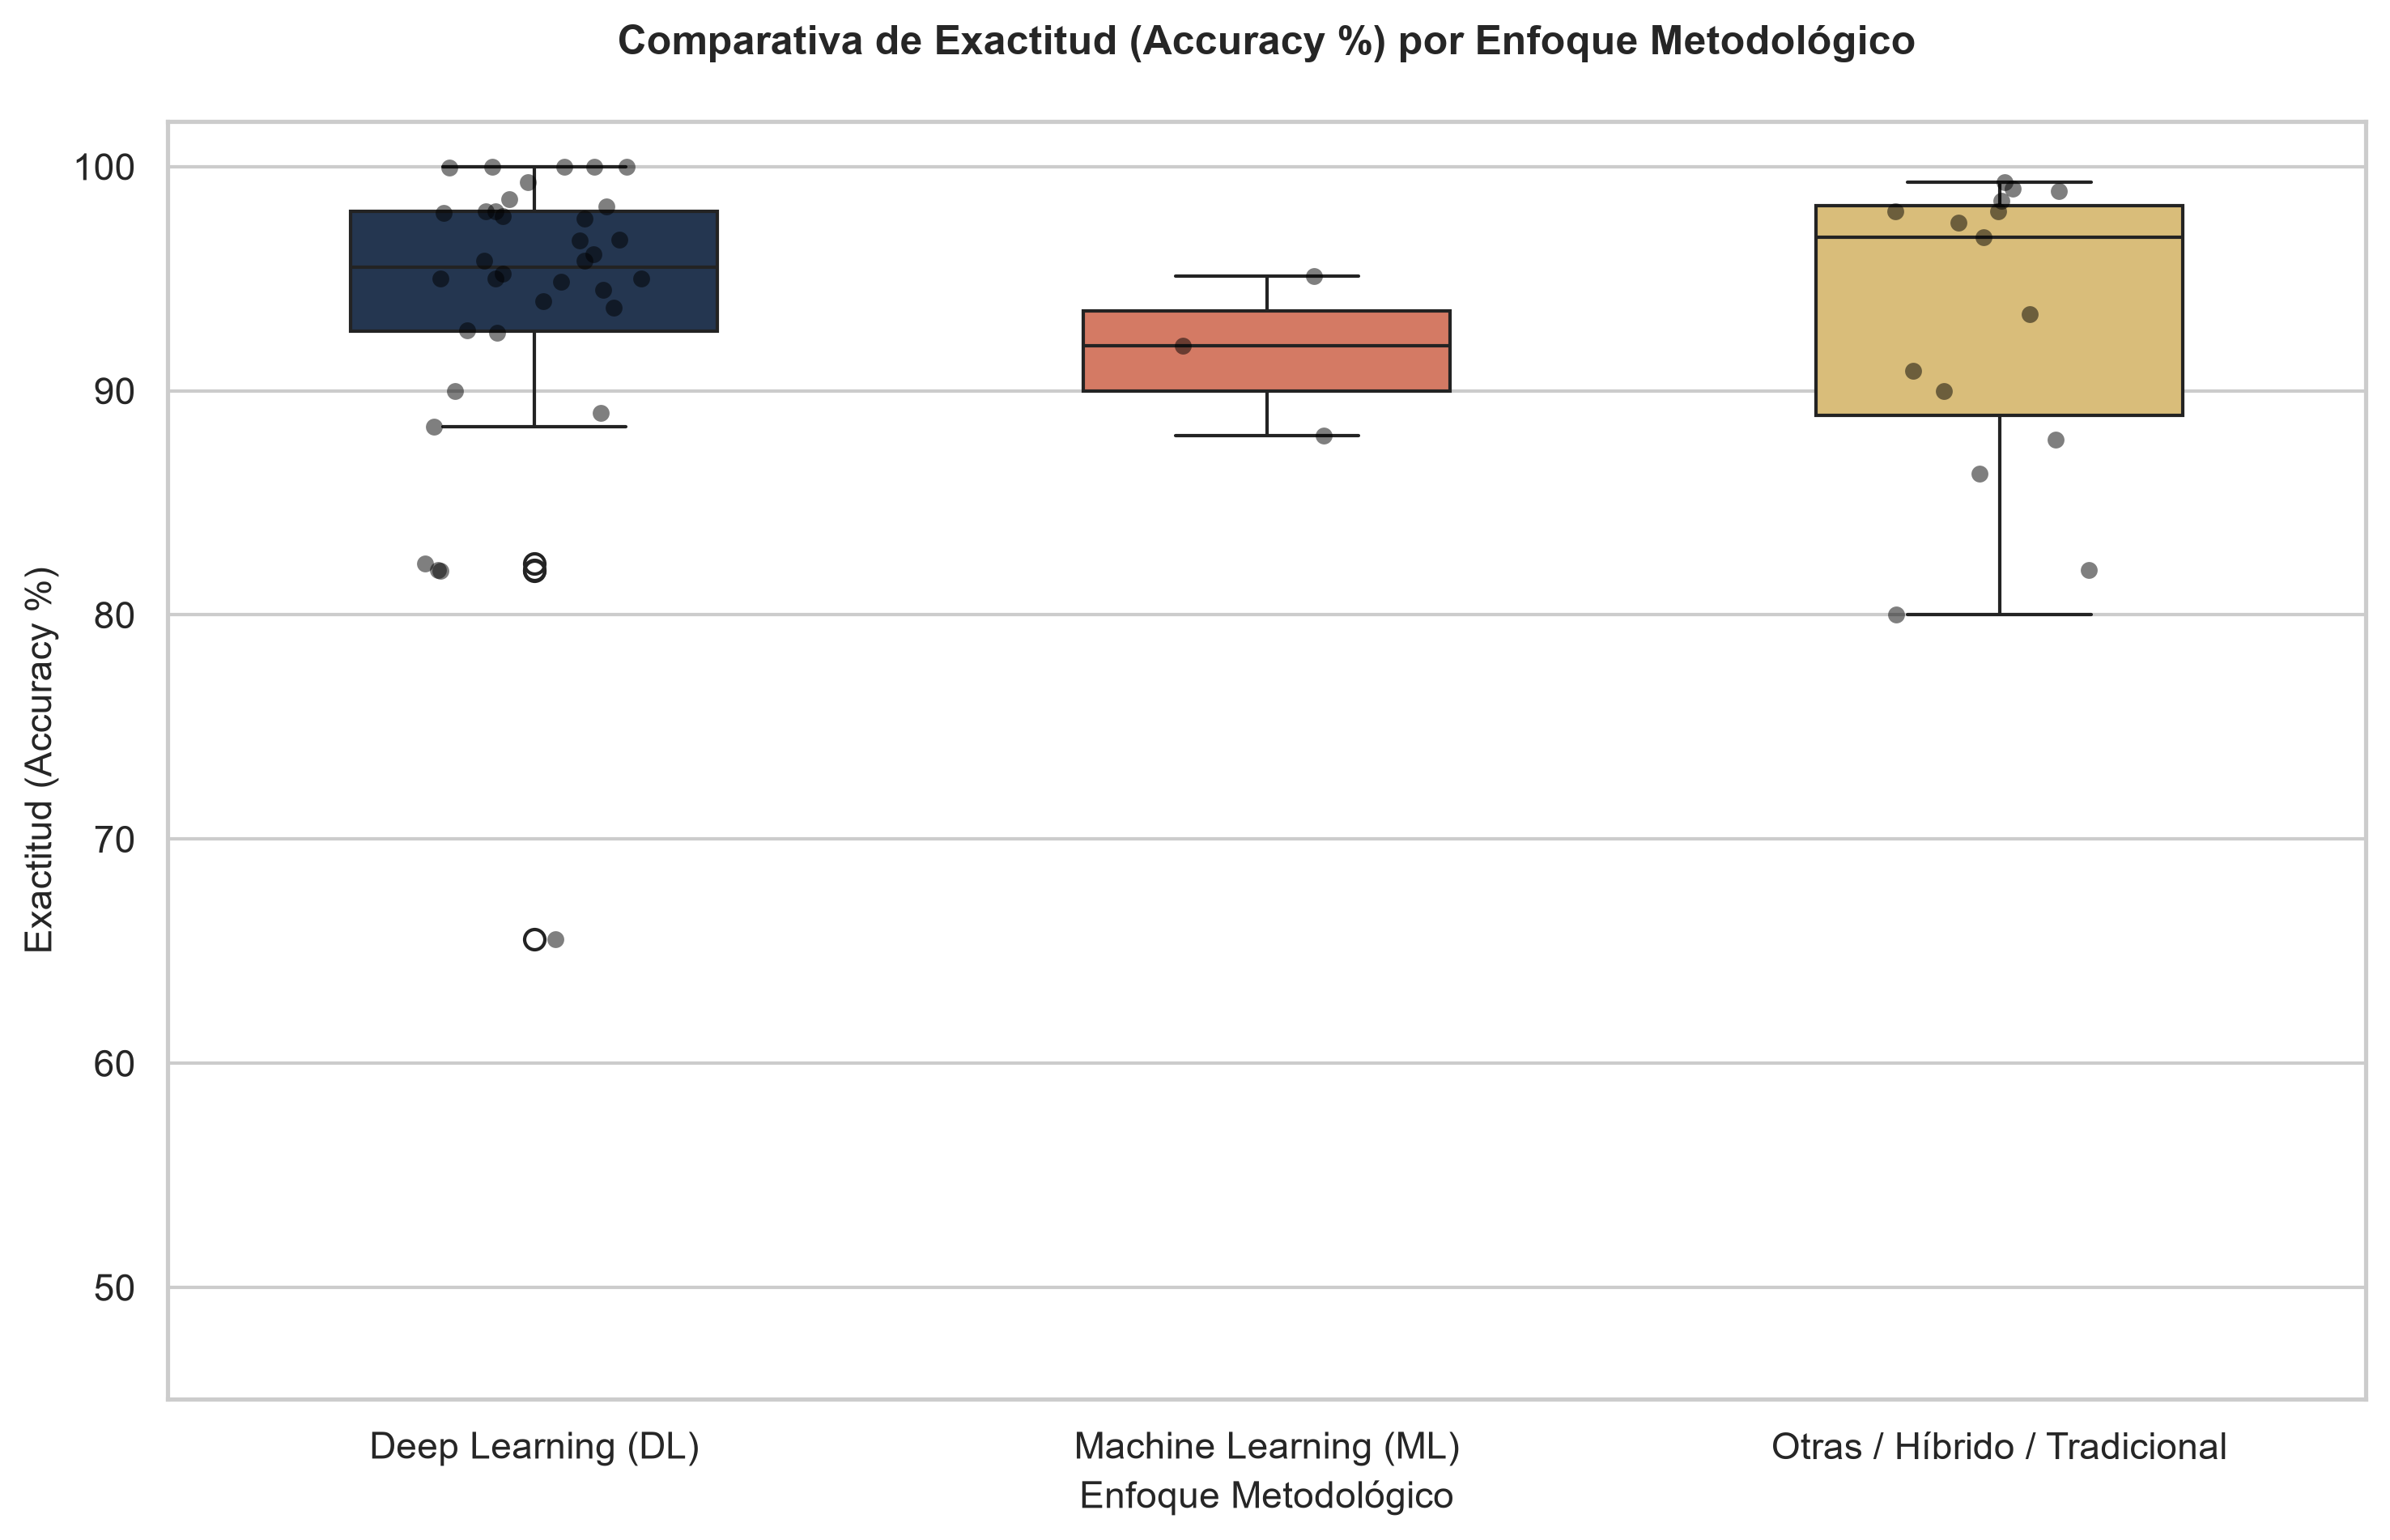
\includegraphics[width=0.48\textwidth]{../graficos/20_boxplot_accuracy_metodologia.png}}
\caption{Comparativa de la Distribución de Exactitud (Accuracy \%) según el Enfoque Metodológico de IA.}
\label{fig:boxplot_accuracy}
\end{figure}

\subsection{Tabulación de Investigaciones Destacadas}
Las Tablas de la \ref{tab:articulos_conductores_1} a la \ref{tab:articulos_conductores_4} y de la \ref{tab:articulos_transporte_1} a la \ref{tab:articulos_transporte_5} presentan el compendio total de las investigaciones analizadas en esta revisión sistemática, detallando la metodología de IA, el entorno experimental y las métricas de rendimiento de cada trabajo.

\begin{table*}[htbp]
\centering
\renewcommand{\arraystretch}{1.1}
\caption{Resumen de Investigaciones en Monitoreo de Conductores y Métricas de Rendimiento (Parte 1)}
\label{tab:articulos_conductores_1}
\footnotesize
\begin{tabular}{cp{7.5cm}p{2.8cm}p{2.8cm}p{2.8cm}}
\toprule
\textbf{Ref.} & \textbf{Título del Trabajo} & \textbf{Metodología IA} & \textbf{Entorno de Prueba} & \textbf{Métrica de Rendimiento} \\
\midrule
\cite{liu2026research} & Research on the Analysis and Recognition System for Dangerous Driving Behaviors Based o... & YOLOv11, CNN (Redes Convoluciona... & Conducción naturalista / Vehícul... & mAP50 of 69.26, accuracy of 65.5... \\
\cite{abarghooei2026driving} & Driving Behavior Classification and Risk Quantification via Multisensor Machine Learnin... & SVM, Machine Learning & Simulador de conducción / Entorn... & 92\% accuracy, 88\% accuracy \\
\cite{hu2026trustworthy} & Trustworthy Driver State Perception via Contextual Interaction-Driven Evidential Vision... & Deep Learning & No especificado & No especificado \\
\cite{zambrano2026monitoring} & Driver Monitoring System Using Computer Vision for Real-Time Detection of Fatigue, Dist... & CNN (Redes Convolucionales), Mob... & Simulador de conducción / Entorn... & 100\% accuracy \\
\cite{rahman2026costeffective} & A Cost-Effective Intelligent Edge-Based Driver Monitoring System for Real-Time Detectio... & No especificado & Conducción naturalista / Vehícul... & No especificado \\
\cite{zia2025advancing} & Advancing Road Safety: A Comprehensive Evaluation of Object Detection Models for Commer... & YOLOv5, Faster R-CNN, RetinaNet,... & No especificado & No especificado \\
\cite{bhavsar2025evaluating} & Evaluating Defensive Driving Behaviour Based on Safe Distance Between Vehicles: A Case ... & No especificado & UAV / Drones & No especificado \\
\cite{kim2025unsupervised} & Unsupervised Learning Approach for Risky Driving Behavior Identification on Expressways... & CNN (Redes Convolucionales), Aut... & No especificado & No especificado \\
\cite{wu2025visual} & Visual Risk-Aware Decision-Making Method for Autonomous Driving & Reinforcement Learning & Simulador de conducción / Entorn... & No especificado \\
\cite{essahraui2025realtime} & Real-Time Driver Drowsiness Detection Using Facial Analysis and Machine Learning Techni... & YOLOv8, YOLOv5, Faster R-CNN, CN... & No especificado & 100\% precision, accuracy of 98.8... \\
\cite{lin2025dangerous} & Dangerous Driving Behavior Detection Based on Computer Vision & CNN (Redes Convolucionales), Tra... & No especificado & No especificado \\
\cite{satya2025utilization} & Utilization of YoloV8 Algorithm for in-Vehicle Video-Based Driver Monitoring System & YOLOv8 & No especificado & 89.6\% precision, 87.2\% recall, 8... \\
\cite{fei2025enhancing} & Enhancing Driving Safety Evaluation Through Correlation Analysis of Driver Behavior & No especificado & Conducción naturalista / Vehícul... & No especificado \\
\cite{yadav2025enhancing} & Enhancing convolutional neural networks in electroencephalogram driver drowsiness detec... & CNN (Redes Convolucionales), Dee... & No especificado & No especificado \\
\cite{xie2025yoloace} & YOLO-ACE: A Vehicle and Pedestrian Detection Algorithm for Autonomous Driving Scenarios... & YOLOv10, YOLO & No especificado & 70.9 FPS \\
\cite{salakapuri2025integrated} & Integrated deep learning framework for driver distraction detection and real-time road ... & YOLO, CNN (Redes Convolucionales... & No especificado & 25 frames per second \\
\cite{uddin2025abnormal} & Abnormal Driving Behavior Detection: A Machine and Deep Learning Based Hybrid Model & Random Forest, ResNet, Efficient... & No especificado & accuracy of 99.3 \\
\cite{nell2025classification} & Classification of Driver Behaviour Using External Observation Techniques for Autonomous... & YOLO & No especificado & No especificado \\
\cite{sorum2025modeling} & Modeling of injury severity of distracted driving accident using statistical and machin... & XGBoost, Machine Learning & No especificado & No especificado \\
\cite{pang2025risk} & Risk Assessment Method for Autonomous Vehicles Violating Safety Common Sense Based on D... & GMM & No especificado & No especificado \\
\cite{zuo2025composite} & Composite Safety Potential Field for Highway Driving Risk Assessment & No especificado & Conducción naturalista / Vehícul... & No especificado \\
\cite{afridi2025multiclass} & A multi-class driver behavior dataset for real-time detection and road safety enhancement & No especificado & No especificado & No especificado \\
\cite{gupta2024deep} & Deep Learning Model for Driver Behavior Detection in Cyber-Physical System-Based Intell... & Deep Learning & No especificado & 94\% accuracy \\
\cite{salbi2024design} & Design and implementation of a driving safety assistant system based on driver behavior & No especificado & No especificado & No especificado \\
\bottomrule
\end{tabular}
\end{table*}


\begin{table*}[htbp]
\centering
\renewcommand{\arraystretch}{1.1}
\caption{Resumen de Investigaciones en Monitoreo de Conductores y Métricas de Rendimiento (Parte 2)}
\label{tab:articulos_conductores_2}
\footnotesize
\begin{tabular}{cp{7.5cm}p{2.8cm}p{2.8cm}p{2.8cm}}
\toprule
\textbf{Ref.} & \textbf{Título del Trabajo} & \textbf{Metodología IA} & \textbf{Entorno de Prueba} & \textbf{Métrica de Rendimiento} \\
\midrule
\cite{zhang2024integrating} & Integrating visual large language model and reasoning chain for driver behavior analysi... & No especificado & No especificado & No especificado \\
\cite{kumar2024nonintrusive} & Nonintrusive Driving Behavior Characterization From Road-Side Cameras & Deep Learning & Videovigilancia / CCTV & 650 ms \\
\cite{lu2024validation} & Validation and Analysis of Driving Safety Assessment Metrics in Real-world Car-Followin... & No especificado & Conducción naturalista / Vehícul... & No especificado \\
\cite{charef2024assessing} & Assessing the driving behaviour of motorcyclists to improve road safety & No especificado & No especificado & No especificado \\
\cite{usman2024distracted} & Detection of distracted driving through the analysis of real-time driver, vehicle, and ... & Random Forest & Simulador de conducción / Entorn... & No especificado \\
\cite{sen2024passive} & Passive Monitoring of Dangerous Driving Behaviors Using mmWave Radar & CNN (Redes Convolucionales) & No especificado & No especificado \\
\cite{liu2024safety} & Safety Driving Detection Based on Convolution Neural Network & YOLOv5, Deep Learning & No especificado & No especificado \\
\cite{qi2024augmented} & Augmented Recognition of Distracted Driving State Based on Electrophysiological Analysi... & XGBoost, Machine Learning & Simulador de conducción / Entorn... & accuracy of 95.1 \\
\cite{wu2024driving} & Driving Attention State Detection Based on GRU-EEGNet & SVM, Deep Learning & No especificado & No especificado \\
\cite{eddine2024investigating} & On investigating drivers’ attention allocation during partially-automated driving & No especificado & Simulador de conducción / Entorn... & No especificado \\
\cite{khattak2024role} & The role of driver head pose dynamics and instantaneous driving in safety critical even... & No especificado & Conducción naturalista / Vehícul... & No especificado \\
\cite{chadha2024enhancing} & Enhancing Road Safety: A Driver Fatigue Detection and Behaviour Monitoring System using... & No especificado & No especificado & No especificado \\
\cite{lin2024realization} & Realization of a Safe Driving Monitoring System for Motor Vehicles & No especificado & No especificado & No especificado \\
\cite{li2024yolosgc} & YOLO-SGC: A Dangerous Driving Behavior Detection Method With Multiscale Spatial-Channel... & YOLOv8, YOLO & No especificado & No especificado \\
\cite{qu2024comprehensive} & Comprehensive study of driver behavior monitoring systems using computer vision and mac... & Machine Learning & No especificado & No especificado \\
\cite{calenzani2024study} & A Study on the Effectiveness of GPT-4V in Classifying Driver Behavior Captured on Video... & No especificado & No especificado & 98.9\% accuracy, 98.4\% accuracy, ... \\
\cite{piruano2024audiovisual} & Audiovisual presentation of variable message signs improves message processing in distr... & No especificado & No especificado & No especificado \\
\cite{komol2024prediction} & Prediction of Drivers' Red-Light Running Behaviour in Connected Vehicle Environments Us... & LSTM & Conducción naturalista / Vehícul... & No especificado \\
\cite{khan2024enhanced} & An Enhanced Deep Neural Network Model for the Detection of Anomalous Behavior of Driver... & YOLOv3, ResNet, MobileNet, Deep ... & No especificado & accuracy of 95 \\
\cite{jebraeily2024drowsiness} & Driver Drowsiness Detection Based on Convolutional Neural Network Architecture Optimiza... & CNN (Redes Convolucionales) & No especificado & No especificado \\
\cite{hernandez2024realtime} & Real-time driver drowsiness and distraction detection using convolutional neural networ... & CNN (Redes Convolucionales) & Conducción naturalista / Vehícul... & No especificado \\
\cite{connie2024wrongway} & Wrong-Way Driving Detection for Enhanced Road Safety using Computer Vision and Machine ... & YOLOv4, Deep Learning, Machine L... & No especificado & No especificado \\
\cite{vamshi2023distracted} & Detection of Distracted Driver Using Convolutional Neural Network & CNN (Redes Convolucionales), Res... & No especificado & No especificado \\
\cite{charly2023identifying} & Identifying risky driving behavior: a field study using instrumented vehicles & No especificado & No especificado & No especificado \\
\bottomrule
\end{tabular}
\end{table*}


\begin{table*}[htbp]
\centering
\renewcommand{\arraystretch}{1.1}
\caption{Resumen de Investigaciones en Monitoreo de Conductores y Métricas de Rendimiento (Parte 3)}
\label{tab:articulos_conductores_3}
\footnotesize
\begin{tabular}{cp{7.5cm}p{2.8cm}p{2.8cm}p{2.8cm}}
\toprule
\textbf{Ref.} & \textbf{Título del Trabajo} & \textbf{Metodología IA} & \textbf{Entorno de Prueba} & \textbf{Métrica de Rendimiento} \\
\midrule
\cite{mulhall2023european} & European NCAP Driver State Monitoring Protocols: Prevalence of Distraction in Naturalis... & No especificado & Conducción naturalista / Vehícul... & No especificado \\
\cite{galloway2023evaluation} & Evaluation of intersection crashes using naturalistic driving data through the lens of ... & No especificado & Conducción naturalista / Vehícul... & No especificado \\
\cite{amini2023distraction} & Driver distraction and in-vehicle interventions: A driving simulator study on visual at... & No especificado & Simulador de conducción / Entorn... & No especificado \\
\cite{xue2023young} & Young Novice Drivers’ Cognitive Distraction Detection: Comparing Support Vector Machine... & SVM, Random Forest & Simulador de conducción / Entorn... & No especificado \\
\cite{zhang2023realtime} & Real-time driving risk assessment based on the psycho-physical field & No especificado & Conducción naturalista / Vehícul... & No especificado \\
\cite{gu2023rfdanet} & RFDANet: an FMCW and TOF radar fusion approach for driver activity recognition using mu... & CNN (Redes Convolucionales), LST... & No especificado & accuracy of 94.5 \\
\cite{ahmed2023deeplearning} & A Deep-Learning Approach to Driver Drowsiness Detection & CNN (Redes Convolucionales) & No especificado & No especificado \\
\cite{majeed2023drowsiness} & Detection of Drowsiness among Drivers Using Novel Deep Convolutional Neural Network Model & CNN (Redes Convolucionales), Dee... & No especificado & accuracy of 96.69 \\
\cite{chen2023visionlanguage} & Vision-Language Models Can Identify Distracted Driver Behavior From Naturalistic Videos & No especificado & Conducción naturalista / Vehícul... & No especificado \\
\cite{domala2023unsafe} & Detection of Unsafe Driving and Drivers Behaviour Monitoring System & Machine Learning & No especificado & No especificado \\
\cite{safarov2023realtime} & Real-Time Deep Learning-Based Drowsiness Detection: Leveraging Computer-Vision and Eye-... & Deep Learning & No especificado & 95.8\% accuracy \\
\cite{fries2023modeling} & Modeling driver behavior in critical traffic scenarios for the safety assessment of aut... & No especificado & Simulador de conducción / Entorn... & No especificado \\
\cite{khosravinia2023enhancing} & Enhancing Road Safety Through Accurate Detection of Hazardous Driving Behaviors With Gr... & No especificado & No especificado & accuracy of 97.5, accuracy of 98.1 \\
\cite{wang2023risk} & Risk Assessment of Distracted Driving Behavior Based on Visual Stability Coefficient & No especificado & Simulador de conducción / Entorn... & No especificado \\
\cite{savkin2022unusual} & Unusual Driver Behavior Detection in Videos Using Deep Learning Models & CNN (Redes Convolucionales), Res... & No especificado & No especificado \\
\cite{wang2022potential} & Potential risk assessment for safe driving of autonomous vehicles under occluded vision & No especificado & No especificado & No especificado \\
\cite{perera2022improving} & Improving EEG-Based Driver Distraction Classification Using Brain Connectivity Estimators & SVM & Simulador de conducción / Entorn... & No especificado \\
\cite{luo2022detecting} & Detecting Driver Cognition Alertness State From Visual Activities in Normal and Emergen... & Deep Learning & No especificado & No especificado \\
\cite{suttiponpisarn2022autonomous} & An Autonomous Framework for Real-Time Wrong-Way Driving Vehicle Detection from Closed-C... & Deep Learning & Videovigilancia / CCTV & 95.23\% accuracy \\
\cite{panwar2022ddnet} & DDNet- A Deep Learning Approach to Detect Driver Distraction and Drowsiness & CNN (Redes Convolucionales), Dee... & No especificado & 99.95\% accuracy \\
\cite{xiao2022attentionbased} & Attention-based deep neural network for driver behavior recognition & No especificado & No especificado & accuracy of 98.48 \\
\cite{haghighat2022computer} & A computer vision‐based deep learning model to detect wrong‐way driving using pan–tilt–... & Deep Learning & Videovigilancia / CCTV & No especificado \\
\cite{minhas2022smart} & A smart analysis of driver fatigue and drowsiness detection using convolutional neural ... & CNN (Redes Convolucionales), Res... & No especificado & 93.69\% accuracy \\
\cite{wang2022intelligent} & Intelligent Detection of Vehicle Driving Safety Based on Deep Learning & YOLO, SSD, CNN (Redes Convolucio... & No especificado & 79.6\% accuracy, 99.96\% accuracy,... \\
\bottomrule
\end{tabular}
\end{table*}


\begin{table*}[htbp]
\centering
\renewcommand{\arraystretch}{1.1}
\caption{Resumen de Investigaciones en Monitoreo de Conductores y Métricas de Rendimiento (Parte 4)}
\label{tab:articulos_conductores_4}
\footnotesize
\begin{tabular}{cp{7.5cm}p{2.8cm}p{2.8cm}p{2.8cm}}
\toprule
\textbf{Ref.} & \textbf{Título del Trabajo} & \textbf{Metodología IA} & \textbf{Entorno de Prueba} & \textbf{Métrica de Rendimiento} \\
\midrule
\cite{dong2022fatigue} & Driver Fatigue and Distracted Driving Detection Using Random Forest and Convolutional N... & CNN (Redes Convolucionales), Ran... & No especificado & No especificado \\
\cite{hossain2022automatic} & Automatic driver distraction detection using deep convolutional neural networks & CNN (Redes Convolucionales), Mob... & No especificado & No especificado \\
\cite{jannusch2021cars} & Cars and distraction: How to address the limits of Driver Monitoring Systems and improv... & No especificado & No especificado & No especificado \\
\cite{papakostas2021understanding} & Understanding Driving Distractions: A Multimodal Analysis on Distraction Characterization & No especificado & No especificado & No especificado \\
\cite{hua2021cognitive} & Cognitive Distraction State Recognition of Drivers at a Nonsignalized Intersection in a... & LSTM, Bi-LSTM, SVM & No especificado & No especificado \\
\cite{chen2021risky} & Risky Driving Behavior Recognition Based on Vehicle Trajectory & No especificado & UAV / Drones & No especificado \\
\cite{shahverdy2021behaviour} & Driver behaviour detection using 1D convolutional neural networks & CNN (Redes Convolucionales) & No especificado & accuracy of 99.999 \\
\cite{garcaherrero2021assessment} & Assessment of the Influence of Technology-Based Distracted Driving on Drivers’ Infracti... & No especificado & No especificado & No especificado \\
\cite{lattanzi2021machine} & Machine Learning Techniques to Identify Unsafe Driving Behavior by Means of In-Vehicle ... & SVM, Machine Learning & No especificado & No especificado \\
\cite{xie2021realtime} & Real-Time Driving Distraction Recognition Through a Wrist-Mounted Accelerometer & CNN (Redes Convolucionales), LSTM & Simulador de conducción / Entorn... & No especificado \\
\cite{shi2021research} & Research on Safe Driving Evaluation Method Based on Machine Vision and Long Short-Term ... & SSD, CNN (Redes Convolucionales)... & No especificado & No especificado \\
\cite{xu2021improvement} & The Improvement of Road Driving Safety Guided by Visual Inattentional Blindness & No especificado & No especificado & No especificado \\
\cite{ameen2021identification} & Identification of Driving Safety Profiles in Vehicle to Vehicle Communication System Ba... & No especificado & No especificado & 90\% accuracy \\
\cite{kezebou2021deep} & A deep neural network approach for detecting wrong-way driving incidents on highway roads & YOLOv5, Deep Learning & Videovigilancia / CCTV & No especificado \\
\cite{sun2020research} & Research on a Cognitive Distraction Recognition Model for Intelligent Driving Systems B... & LSTM, Bi-LSTM, SVM & Conducción naturalista / Vehícul... & No especificado \\
\cite{niu2020study} & Study on drivers' visual perception characteristics during the take‐over of vehicle con... & No especificado & Simulador de conducción / Entorn... & No especificado \\
\cite{he2020influence} & The Influence of Visual-Manual Distractions on Anticipatory Driving & No especificado & Simulador de conducción / Entorn... & No especificado \\
\cite{lattanzi2020improving} & Improving Machine Learning Identification of Unsafe Driver Behavior by Means of Sensor ... & SVM, Machine Learning & No especificado & accuracy of 88 \\
\cite{sheykhfard2020distraction} & Driver distraction by digital billboards? Structural equation modeling based on natural... & No especificado & Conducción naturalista / Vehícul... & No especificado \\
\cite{shahverdy2020behavior} & Driver behavior detection and classification using deep convolutional neural networks & CNN (Redes Convolucionales), Dee... & No especificado & No especificado \\
\cite{huang2020hybrid} & HCF: A Hybrid CNN Framework for Behavior Detection of Distracted Drivers & CNN (Redes Convolucionales), Res... & No especificado & accuracy of 96.74 \\
\cite{ouyang2020deep} & Deep CNN-Based Real-Time Traffic Light Detector for Self-Driving Vehicles & CNN (Redes Convolucionales), Dee... & Conducción naturalista / Vehícul... & accuracy of 99.3 \\
\bottomrule
\end{tabular}
\end{table*}




\begin{table*}[htbp]
\centering
\renewcommand{\arraystretch}{1.1}
\caption{Resumen de Investigaciones en Detección de Infracciones y Accidentes de Tránsito (Parte 1)}
\label{tab:articulos_transporte_1}
\footnotesize
\begin{tabular}{cp{7.5cm}p{2.8cm}p{2.8cm}p{2.8cm}}
\toprule
\textbf{Ref.} & \textbf{Título del Trabajo} & \textbf{Metodología IA} & \textbf{Entorno de Prueba} & \textbf{Métrica de Rendimiento} \\
\midrule
\cite{l2026safestreets} & SafeStreets: Deep Learning-Based Real-Time Traffic Violation Detection System & CNN (Redes Convolucionales), Dee... & Videovigilancia / CCTV & No especificado \\
\cite{kumar2026intelligent} & Intelligent Traffic Accident Detection System using Deep Learning Fusion Techniques & LSTM, Transformer, ResNet, Deep ... & Videovigilancia / CCTV & accuracy of 97.93 \\
\cite{ahmad2026comparative} & A Comparative Evaluation of Deep Learning Models for Road Accident Detection Using CCTV... & CNN (Redes Convolucionales), LST... & Videovigilancia / CCTV & 99\% accuracy, 99.53\% accuracy \\
\cite{kumar2026uavbased} & UAV-based object detection model for smart surveillance using deep neural network & YOLOv5 & UAV / Drones & 95.1 \% precision, 86.3 \% recall \\
\cite{chen2026hybrid} & Hybrid Deep Learning and Classification Framework for Automatic Traffic Inspection Clas... & YOLOv5, CNN (Redes Convolucional... & No especificado & No especificado \\
\cite{srivastava2026traffic} & Traffic Violations Control Using Deep Learning & Deep Learning & Videovigilancia / CCTV & accuracy of 0.927 \\
\cite{pavan2026aipowered} & AI-Powered Traffic Violation Detection System Using CCTV, and Deep Learning & YOLOv8, Deep Learning & Videovigilancia / CCTV & accuracy of 88.4, 28 FPS, 180 ms \\
\cite{yang2025computer} & Computer Vision-Based Traffic Monitoring: Design of a Red-Light Violation Detection Sys... & YOLOv5, Deep Learning & No especificado & 95\% accuracy \\
\cite{jing2025traffic} & Traffic Incident Detection Algorithm based on Deep Learning: A Statistical Optimization... & YOLOv5, Deep Learning & No especificado & No especificado \\
\cite{le2025redlight} & Red-light Running Detection & YOLOv8, YOLO, CNN (Redes Convolu... & Videovigilancia / CCTV & 89.2\% precision, 92.6\% recall \\
\cite{silva2025light} & Red Light Running Detection Using AI-Powered Object Tracking on Embedded Systems & YOLOv8, CNN (Redes Convolucionales) & No especificado & 29 fps \\
\cite{oussouaddi2025dsryolo} & DSR-YOLO: A Lightweight and Efficient YOLOv8 Model for Enhanced Pedestrian Detection & YOLOv8, YOLO & No especificado & No especificado \\
\cite{abukhadrah2025droneassisted} & Drone-assisted adaptive object detection and privacy-preserving surveillance in smart c... & Reinforcement Learning & UAV / Drones & No especificado \\
\cite{deshpande2025computervision} & Computer-vision based automatic rider helmet violation detection and vehicle identifica... & YOLOv8, CNN (Redes Convolucional... & No especificado & accuracy of 98.56 \\
\cite{elhenidy2025gyyolo} & GY-YOLO: ghost separable YOLO for pedestrian detection & YOLOv8, YOLOv5, YOLO & Videovigilancia / CCTV & 92.8\% mAp, 90.3\% mAp, 91.1\% mAp \\
\cite{barbu2025deep} & Deep Learning-based Multiple Pedestrian Crossing Behavior Analysis Framework & YOLO, CNN (Redes Convolucionales... & No especificado & No especificado \\
\cite{chouhan2025deep} & Deep Learning based enhanced aerial object detection & Deep Learning & UAV / Drones & No especificado \\
\cite{singh2025realtime} & Real-time Identification of Traffic Violations through Deep Learning Techniques & Deep Learning & No especificado & accuracy of 95.8 \\
\cite{huang2025dtldetector} & D-TLDetector: Advancing Traffic Light Detection With a Lightweight Deep Learning Model & Transformer, Vision Transformer ... & No especificado & 98.23\% accuracy, 135 FPS \\
\cite{alshehri2025integrated} & Integrated neural network framework for multi-object detection and recognition using UA... & YOLOv11, LSTM, Autoencoder, Tran... & UAV / Drones & accuracy of 97.8, accuracy of 96... \\
\cite{mota2025integration} & Integration of deep learning algorithms for real-time vehicle accident detection from s... & CNN (Redes Convolucionales), Res... & Videovigilancia / CCTV & accuracy of 98 \\
\cite{kavitha2025towards} & Towards Safer Roads: An End-to-End Deep Learning Framework for Traffic Violation Detect... & YOLOv8, Deep Learning & No especificado & No especificado \\
\cite{rachoti2025traffic} & Traffic Detection and Traffic Violation Detection using Deep Learning: An End-to-End YO... & YOLO, Deep Learning & Videovigilancia / CCTV & No especificado \\
\cite{abdullah2025lcyolo} & LC-YOLO: An Improved YOLOv8-Based Lane Detection Model for Enhanced Lane Intrusion Dete... & YOLOv8, YOLO, Deep Learning & No especificado & 97.9\% mAP, mAP of 97.9 \\
\bottomrule
\end{tabular}
\end{table*}


\begin{table*}[htbp]
\centering
\renewcommand{\arraystretch}{1.1}
\caption{Resumen de Investigaciones en Detección de Infracciones y Accidentes de Tránsito (Parte 2)}
\label{tab:articulos_transporte_2}
\footnotesize
\begin{tabular}{cp{7.5cm}p{2.8cm}p{2.8cm}p{2.8cm}}
\toprule
\textbf{Ref.} & \textbf{Título del Trabajo} & \textbf{Metodología IA} & \textbf{Entorno de Prueba} & \textbf{Métrica de Rendimiento} \\
\midrule
\cite{bhaskara2025deep} & Deep Learning-based Traffic Violation Detection using YOLOv8 and PaddleOCR & YOLOv8, Deep Learning & No especificado & No especificado \\
\cite{suresh2025traffic} & Traffic Violation Detection Using Deep Learning & YOLO, CNN (Redes Convolucionales... & No especificado & No especificado \\
\cite{owais2025light} & Red light crossing violations modelling using deep learning and variance-based sensitiv... & Deep Learning & No especificado & No especificado \\
\cite{gowroju2025urbaneye} & UrbanEye: Deep Learning Enhanced Two-Wheeler Traffic Rule Violation Detection using YOL... & YOLO, Deep Learning & No especificado & No especificado \\
\cite{pujitha2025traffic} & Traffic Signal Violation Detection System & SSD, CNN (Redes Convolucionales)... & No especificado & No especificado \\
\cite{balasaranya2025realtime} & Real-Time Traffic Violation Detection with Automated Enforcement Using Computer Vision & YOLOv5, Mask R-CNN, CNN (Redes C... & No especificado & No especificado \\
\cite{ijaradar2025datadriven} & Data-Driven Anomaly Detection in Urban Traffic Data: A Deep Learning Approach & LSTM, Autoencoder, Deep Learning & No especificado & No especificado \\
\cite{wang2025application} & Application and Optimization of Convolutional Neural Networks Based on Deep Learning in... & CNN (Redes Convolucionales), Dee... & No especificado & No especificado \\
\cite{kumar2025smart} & The Smart City Transportation: Deep Learning Ensemble Approach for Traffic Accident Det... & CNN (Redes Convolucionales), Tra... & Videovigilancia / CCTV & No especificado \\
\cite{kalwa2025unusual} & Detection of Unusual Activities on the Road Using Deep CNN & CNN (Redes Convolucionales), Dee... & No especificado & No especificado \\
\cite{duan2025multimodal} & A multimodal deep fusion framework for highway traffic anomaly detection & LSTM & No especificado & accuracy of 0.980, F1 score of 0... \\
\cite{vazquezmonjaras2024unsafe} & Detection of Unsafe Behavior in conveying Vehicle Parts using Computer Vision & YOLOv8, CNN (Redes Convolucional... & Entorno industrial / Laboral & No especificado \\
\cite{nal2024unsafenet} & Unsafe-Net: YOLO v4 and ConvLSTM based computer vision system for real-time detection o... & YOLO, Deep Learning & Entorno industrial / Laboral & No especificado \\
\cite{ren2024intelligent} & Intelligent Vehicle Violation Detection System Under Human–Computer Interaction and Com... & No especificado & No especificado & 96.86\% accuracy \\
\cite{liu2024network} & IoT Network Traffic Analysis with Deep Learning & Deep Learning, Machine Learning & No especificado & 98\% accuracy \\
\cite{thomas2024automated} & Automated Detection of Traffic Rule Violation using Deep Learning Techniques & YOLOv5, Deep Learning & No especificado & accuracy of 90 \\
\cite{poudel2024improved} & Improved Object Detection in UAV Images using Deep Learning & YOLOv5, Deep Learning & UAV / Drones & No especificado \\
\cite{michielsen2024historybased} & History-Based Road Traffic Anomaly Detection Using Deep Learning and Real-World Data & Deep Learning & No especificado & No especificado \\
\cite{arjunan2024realtime} & Real-Time Detection of Network Traffic Anomalies in Big Data Environments Using Deep Le... & CNN (Redes Convolucionales), LST... & No especificado & No especificado \\
\cite{driessen2024putting} & Putting ChatGPT vision (GPT-4V) to the test: risk perception in traffic images & No especificado & No especificado & No especificado \\
\cite{m2024traffic} & Traffic Rules Violation Detection System using YOLO v8 Model & YOLO, CNN (Redes Convolucionales) & No especificado & No especificado \\
\cite{li2024dense} & Dense Pedestrian Detection Based on GR-YOLO & YOLOv8, YOLO, Deep Learning & No especificado & No especificado \\
\cite{gehani2024traffic} & Traffic Signal Violation Detection System Using Computer Vision & YOLOv8, Deep Learning & Videovigilancia / CCTV & No especificado \\
\cite{bakirci2024enhancing} & Enhancing vehicle detection in intelligent transportation systems via autonomous UAV pl... & YOLOv8 & UAV / Drones & No especificado \\
\bottomrule
\end{tabular}
\end{table*}


\begin{table*}[htbp]
\centering
\renewcommand{\arraystretch}{1.1}
\caption{Resumen de Investigaciones en Detección de Infracciones y Accidentes de Tránsito (Parte 3)}
\label{tab:articulos_transporte_3}
\footnotesize
\begin{tabular}{cp{7.5cm}p{2.8cm}p{2.8cm}p{2.8cm}}
\toprule
\textbf{Ref.} & \textbf{Título del Trabajo} & \textbf{Metodología IA} & \textbf{Entorno de Prueba} & \textbf{Métrica de Rendimiento} \\
\midrule
\cite{tran2024transformerbased} & Transformer-Based Spatio-Temporal Unsupervised Traffic Anomaly Detection in Aerial Videos & Transformer, Machine Learning & UAV / Drones & No especificado \\
\cite{udayanti2024convolutional} & Convolutional Neural Network and LSTM for Seat Belt Detection in Vehicles using YOLO3 & CNN (Redes Convolucionales), LST... & Videovigilancia / CCTV & 89\% accuracy, accuracy of 89 \\
\cite{shoman2024enforcing} & Enforcing Traffic Safety: A Deep Learning Approach for Detecting Motorcyclists' Helmet ... & YOLOv8, Deep Learning & No especificado & F1 score of 0.91, F1 score of 0.96 \\
\cite{h2024traffic} & Detection of Traffic Violation and Vechicle Number Plate Using Computer Vision & Deep Learning & No especificado & No especificado \\
\cite{tahir2024pvswinyolovs} & PVswin-YOLOv8s: UAV-Based Pedestrian and Vehicle Detection for Traffic Management in Sm... & YOLOv8, YOLOv5, YOLOv3, YOLO, Re... & UAV / Drones & No especificado \\
\cite{samonte2024grand} & Grand challenge of image processing in automatic detection of vehicles running in red l... & No especificado & No especificado & No especificado \\
\cite{khalaf2024deep} & Deep Learning-Based Anomaly Detection in Network Traffic for Cyber Threat Identification & CNN (Redes Convolucionales), Aut... & No especificado & 95\% accuracy \\
\cite{ogundokun2024development} & Development of a Deep Learning-Based System for Road Traffic Anomaly Detection & CNN (Redes Convolucionales), Dee... & No especificado & 100\% accuracy, accuracy of 100 \\
\cite{hernndezdaz2024computer} & A computer vision system for detecting motorcycle violations in pedestrian zones & YOLOv8, SSD, MobileNet, Deep Lea... & Videovigilancia / CCTV & No especificado \\
\cite{almahadin2024vanet} & VANET Network Traffic Anomaly Detection Using GRU-Based Deep Learning Model & Deep Learning & No especificado & No especificado \\
\cite{fakhrurroja2024visionbased} & A Vision-Based System: Detecting Traffic Law Violation Case Study of Red-Light Running ... & YOLOv8, Machine Learning & No especificado & No especificado \\
\cite{shaik2024optimal} & Optimal deep learning based object detection for pedestrian and anomaly recognition model & YOLOv5, CNN (Redes Convolucional... & No especificado & AUC score of 99.05 \\
\cite{wu2024deep} & A deep learning-based car accident detection approach in video-based traffic surveillance & CNN (Redes Convolucionales), Dee... & No especificado & No especificado \\
\cite{bartolomhornillos2024selfadaptive} & A Self-Adaptive Automatic Incident Detection System for Road Surveillance Based on Deep... & Deep Learning & No especificado & accuracy of 2 \\
\cite{natha2024improving} & Improving Traffic Surveillance: Deep Learning Approach for Road Anomaly Detection in Vi... & CNN (Redes Convolucionales), Dee... & Videovigilancia / CCTV & No especificado \\
\cite{yazdani2023intelligent} & Intelligent vehicle pedestrian light (IVPL): A deep reinforcement learning approach for... & Reinforcement Learning & No especificado & No especificado \\
\cite{qu2023pedestrian} & Pedestrian Red-Light Violation Detection Based on Deep Learning Vision & YOLOv5, Deep Learning & No especificado & No especificado \\
\cite{fernandez2023automated} & Automated detection of vehicles with anomalous trajectories in traffic surveillance videos & Deep Learning & Videovigilancia / CCTV & No especificado \\
\cite{hu2023research} & Research on Anomaly Network Detection Based on Self-Attention Mechanism & LSTM, XGBoost, Machine Learning & No especificado & No especificado \\
\cite{tahir2023realtime} & Real-Time Event-Driven Road Traffic Monitoring System Using CCTV Video Analytics & CNN (Redes Convolucionales) & Videovigilancia / CCTV & accuracy of 82.3 \\
\cite{ahn2023deep} & Deep learning-based anomaly detection for individual drone vehicles performing swarm mi... & Deep Learning & UAV / Drones & No especificado \\
\cite{tangamus2023method} & Method For Traffic Violation Detection Using Deep Learning & YOLOv8, CNN (Redes Convolucional... & Videovigilancia / CCTV & No especificado \\
\cite{pradana2023endtoend} & An End-to-End Online Traffic-Risk Incident Prediction in First-Person Dash Camera Videos & No especificado & No especificado & 9.60 fps, 1.44 fps \\
\cite{mastouri2023contextaware} & A Context-Aware, Computer-Vision-Based Approach for the Detection of Taxi Street-Hailin... & No especificado & Entorno industrial / Laboral & 80\% accuracy, 84\% precision, 84\%... \\
\bottomrule
\end{tabular}
\end{table*}


\begin{table*}[htbp]
\centering
\renewcommand{\arraystretch}{1.1}
\caption{Resumen de Investigaciones en Detección de Infracciones y Accidentes de Tránsito (Parte 4)}
\label{tab:articulos_transporte_4}
\footnotesize
\begin{tabular}{cp{7.5cm}p{2.8cm}p{2.8cm}p{2.8cm}}
\toprule
\textbf{Ref.} & \textbf{Título del Trabajo} & \textbf{Metodología IA} & \textbf{Entorno de Prueba} & \textbf{Métrica de Rendimiento} \\
\midrule
\cite{golcarenarenji2023robust} & Robust real-time traffic light detector on small-form platform for autonomous vehicles & CNN (Redes Convolucionales), Mac... & No especificado & 93.42\% accuracy, 30.01 Frames Pe... \\
\cite{chaturvedi2023traffic} & Detection of traffic rule violation in University campus using deep learning model & YOLO, Deep Learning & Videovigilancia / CCTV & No especificado \\
\cite{wang2023network} & Network Anomaly Intrusion Detection Based on Deep Learning Approach & CNN (Redes Convolucionales), LST... & No especificado & No especificado \\
\cite{madhavi2023traffic} & Traffic Congestion Detection from Surveillance Videos using Deep Learning & CNN (Redes Convolucionales), Dee... & Videovigilancia / CCTV & No especificado \\
\cite{adewopo2023smart} & Smart City Transportation: Deep Learning Ensemble Approach for Traffic Accident Detection & Deep Learning & No especificado & No especificado \\
\cite{uvais2023traffic} & Traffic Signal Violation Detection Through Computer Vision & Deep Learning & No especificado & No especificado \\
\cite{zahid2023datadriven} & A data-driven approach for road accident detection in surveillance videos & CNN (Redes Convolucionales), Res... & Simulador de conducción / Entorn... & No especificado \\
\cite{winter2023predicting} & Predicting perceived risk of traffic scenes using computer vision & No especificado & No especificado & No especificado \\
\cite{mane2023realtime} & Real-Time Vehicle Accident Recognition from Traffic Video Surveillance using YOLOV8 and... & YOLOv8 & No especificado & 93.8\% precision, 98\% recall, 96.... \\
\cite{ahmed2023realtime} & A Real-Time Computer Vision Based Approach to Detection and Classification of Traffic I... & YOLOv5, ResNet & No especificado & mAP of 83.3 \\
\cite{tamagusko2022deep} & Deep Learning applied to Road Accident Detection with Transfer Learning and Synthetic I... & Deep Learning & No especificado & No especificado \\
\cite{zhu2022deep} & Deep learning for autonomous vehicle and pedestrian interaction safety & CNN (Redes Convolucionales), Dee... & No especificado & accuracy of 81.98 \\
\cite{lavingia2022machine} & Machine Learning Based Approach for Traffic Rule Violation Detection & YOLOv3, Deep Learning, Machine L... & No especificado & No especificado \\
\cite{du2022improvement} & Improvement of Lightweight Convolutional Neural Network Model Based on YOLO Algorithm a... & YOLOv5, YOLOv3, YOLO, CNN (Redes... & No especificado & No especificado \\
\cite{chen2022research} & Research on Pedestrian Detection and DeepSort Tracking in Front of Intelligent Vehicle ... & YOLO, Deep Learning & No especificado & No especificado \\
\cite{yasamorn2022object} & Object Detection of Pedestrian Crossing Accident Using Deep Convolutional Neural Networks & YOLOv3, Faster R-CNN, CNN (Redes... & Videovigilancia / CCTV & No especificado \\
\cite{cypto2022automatic} & Automatic detection system of speed violations in a traffic based on deep learning tech... & YOLO, Deep Learning & No especificado & No especificado \\
\cite{alqubaydhi2022unauthorized} & Detection of Unauthorized Unmanned Aerial Vehicles Using YOLOv5 and Transfer Learning & YOLOv5 & UAV / Drones & No especificado \\
\cite{thao2022automatic} & Automatic Traffic Red-Light Violation Detection Using AI & YOLOv5, Machine Learning & No especificado & 86\% accuracy, accuracy of 82 \\
\cite{arshad2022twowheeler} & Detection of Two-Wheeler Traffic Rule Violation Using Deep Learning & YOLOv5, RetinaNet, Deep Learning & No especificado & 92.6\% accuracy, accuracy of 92.6 \\
\cite{khan2022anomaly} & Anomaly Detection in Traffic Surveillance Videos Using Deep Learning & CNN (Redes Convolucionales), Dee... & Videovigilancia / CCTV & accuracy of 82 \\
\cite{ghahremannezhad2022realtime} & Real-Time Accident Detection in Traffic Surveillance Using Deep Learning & YOLOv4, Deep Learning & Videovigilancia / CCTV & No especificado \\
\cite{zhu2022traffic} & Traffic sign recognition based on deep learning & YOLOv5, SSD, CNN (Redes Convoluc... & No especificado & 90.14\% mAP, 97.70\% mAP \\
\cite{fedosov2021method} & Method For Detecting Violation at a Pedestrian Crossing Using a Convolutional Neuaral N... & YOLO, CNN (Redes Convolucionales) & No especificado & No especificado \\
\bottomrule
\end{tabular}
\end{table*}


\begin{table*}[htbp]
\centering
\renewcommand{\arraystretch}{1.1}
\caption{Resumen de Investigaciones en Detección de Infracciones y Accidentes de Tránsito (Parte 5)}
\label{tab:articulos_transporte_5}
\footnotesize
\begin{tabular}{cp{7.5cm}p{2.8cm}p{2.8cm}p{2.8cm}}
\toprule
\textbf{Ref.} & \textbf{Título del Trabajo} & \textbf{Metodología IA} & \textbf{Entorno de Prueba} & \textbf{Métrica de Rendimiento} \\
\midrule
\cite{ahmed2021unmanned} & Unmanned Aerial Multi-Object Dynamic Frame Detection and Skipping Using Deep Learning o... & Deep Learning & UAV / Drones & No especificado \\
\cite{pillai2021realtime} & Real-time image enhancement for an automatic automobile accident detection through CCTV... & YOLO, SVM, Deep Learning, Machin... & Videovigilancia / CCTV & 28 frames per second, 12.73 ms \\
\cite{aversano2021effective} & Effective Anomaly Detection Using Deep Learning in IoT Systems & Autoencoder, Deep Learning & No especificado & No especificado \\
\cite{pawar2021deep} & Deep learning based detection and localization of road accidents from traffic surveilla... & Deep Learning & No especificado & No especificado \\
\cite{tattari2021deep} & Deep Neural Networks Based Object Detection for Road Safety Using YOLO-V3 & YOLO, CNN (Redes Convolucionales... & Videovigilancia / CCTV & accuracy of 86.3 \\
\cite{boukerche2021object} & Object Detection Using Deep Learning Methods in Traffic Scenarios & Deep Learning & No especificado & No especificado \\
\cite{dong2021network} & Network Abnormal Traffic Detection Model Based on Semi-Supervised Deep Reinforcement Le... & Autoencoder, Machine Learning, R... & No especificado & No especificado \\
\cite{gupta2021monitoring} & Monitoring and surveillance of urban road traffic using low altitude drone images: a de... & YOLOv4, YOLOv3, SSD, Deep Learning & UAV / Drones & No especificado \\
\cite{aboah2021visionbased} & A Vision-based System for Traffic Anomaly Detection using Deep Learning and Decision Trees & YOLOv5, Deep Learning & Videovigilancia / CCTV & F1 score of 0.8571 \\
\cite{roblesserrano2021automatic} & Automatic Detection of Traffic Accidents from Video Using Deep Learning Techniques & Deep Learning & No especificado & 98\% accuracy, accuracy of 98 \\
\cite{yu2020scenegraph} & Scene-Graph Augmented Data-Driven Risk Assessment of Autonomous Vehicle Decisions & No especificado & No especificado & 70.3\% accuracy, accuracy of 87.8 \\
\cite{svrd2020response} & Detection and response to critical lead vehicle deceleration events with peripheral vis... & No especificado & No especificado & No especificado \\
\cite{franklin2020traffic} & Traffic Signal Violation Detection using Artificial Intelligence and Deep Learning & YOLOv3, Deep Learning & No especificado & accuracy of 97.67, accuracy of 8... \\
\cite{kumaran2020anomaly} & Anomaly Detection in Road Traffic Using Visual Surveillance & Deep Learning & Conducción naturalista / Vehícul... & No especificado \\
\cite{tonge2020traffic} & Traffic Rules Violation Detection using Deep Learning & YOLO, Mask R-CNN, CNN (Redes Con... & No especificado & No especificado \\
\cite{hwang2020unsupervised} & An Unsupervised Deep Learning Model for Early Network Traffic Anomaly Detection & CNN (Redes Convolucionales), Aut... & No especificado & 100\% accuracy \\
\cite{amma2020anomaly} & Anomaly detection framework for Internet of things traffic using vector convolutional d... & Deep Learning & No especificado & No especificado \\
\cite{micheal2020object} & Object Detection and Tracking with UAV Data Using Deep Learning & LSTM, Deep Learning & UAV / Drones & No especificado \\
\cite{wei2020adoption} & Adoption and realization of deep learning in network traffic anomaly detection device d... & CNN (Redes Convolucionales), Dee... & No especificado & No especificado \\
\cite{paweczyk2020real} & Real World Object Detection Dataset for Quadcopter Unmanned Aerial Vehicle Detection & Machine Learning & UAV / Drones & No especificado \\
\cite{reddy2020deep} & Deep neural network based anomaly detection in Internet of Things network traffic track... & Deep Learning, Machine Learning & No especificado & No especificado \\
\cite{chriki2020deep} & Deep learning and handcrafted features for one-class anomaly detection in UAV video & CNN (Redes Convolucionales), SVM... & UAV / Drones & No especificado \\
\cite{kwon2020dynamic} & Dynamic All-Red Signal Control Based on Deep Neural Network Considering Red Light Runne... & CNN (Redes Convolucionales) & No especificado & No especificado \\
\bottomrule
\end{tabular}
\end{table*}




\subsection{Respuestas a las Preguntas de Investigación}
A partir del análisis cuantitativo y cualitativo llevado a cabo en esta revisión, se da respuesta formal a las preguntas de investigación planteadas en la metodología:
\begin{itemize}
    \item \textbf{Respuesta a la PI1 (Paradigmas Tecnológicos):} Se evidencia una hegemonía del Aprendizaje Profundo (Deep Learning), representando el 72.3\% del corpus analizado (135 trabajos). Las arquitecturas de una sola etapa (particularmente la familia YOLO) dominan las tareas de detección de infracciones y objetos viales, mientras que las redes convolucionales combinadas con modelos temporales (LSTM y Transformers) prevalecen en el monitoreo de fatiga y distracción debido a su capacidad para procesar dependencias espaciotemporales de video.
    \item \textbf{Respuesta a la PI2 (Entornos y Despliegue):} Aunque la mayoría de los estudios no detallan su entorno experimental en la base de datos de origen, entre aquellos que sí lo especifican destacan los sistemas de videovigilancia CCTV (30 artículos) y las tecnologías aéreas basadas en drones/UAV (18 artículos) para la gestión de tráfico urbano. La validación para monitoreo de conductores se realiza mayoritariamente en entornos reales de conducción naturalista (18 artículos) y simuladores virtuales (15 artículos). El despliegue de hardware está liderado por dispositivos en el borde como NVIDIA Jetson y Raspberry Pi, implementados mediante librerías OpenCV y MediaPipe.
    \item \textbf{Respuesta a la PI3 (Desafíos y Direcciones Futuras):} Las limitaciones más recurrentes reportadas por los investigadores se centran en la alta sensibilidad de los modelos a variaciones de iluminación extrema (conducción nocturna, deslumbramiento) y oclusiones físicas. Adicionalmente, el resguardo de la privacidad del conductor representa un reto regulatorio crítico. El trabajo futuro en el área apunta al uso de Inteligencia Artificial Explicable (XAI), técnicas de Adaptación de Dominio No Supervisada (UDA), Aprendizaje Federado y fusión multimodal de sensores.
\end{itemize}
